\documentclass[11pt,a4paper]{article}
\usepackage[utf8]{inputenc}
\usepackage[T1]{fontenc}
\usepackage{amsfonts}
\usepackage[french]{babel}
\frenchbsetup{StandardLists=true} % à inclure si on utilise \usepackage[francais]{babel}
\usepackage{enumitem}
\usepackage{amssymb}
\usepackage{amsmath}
\usepackage[left=2cm,right=2cm,top=2cm,bottom=2cm]{geometry}
\usepackage{multirow}
\usepackage[dvipsnames]{xcolor}

\usepackage[T1]{fontenc}
\usepackage{fouriernc}
\usepackage{graphicx}

\usepackage{setspace}
\singlespacing

\usepackage{multicol}
\usepackage{caption}
\usepackage{fancyhdr}
\pagestyle{fancy}
\renewcommand\headrulewidth{1pt}
\fancyhead[L]{Lycée Denis Diderot }
\fancyhead[R]{Classe de Terminale}
\setcounter{page}{1}\fancyfoot[C]{page \thepage}
\fancyfoot[R]{Année 2025 2026}
\fancyfoot[L]{Alexis RUIZ}
\usepackage{multirow,tabularx,booktabs}
\newcommand{\cadreblanc}[1]{%
\medskip\framebox[\linewidth][c]{%
\rule{0mm}{#1mm}}\par
\medskip}

\setlength{\columnseprule}{0.2pt} 

\renewcommand{\arraystretch}{2}
\newcommand*\acocher{\quitvmode{\fboxsep0pt \fboxrule0.8pt \fbox{\vrule height1.8ex depth.1ex width0pt \vrule height0pt depth0pt width1.9ex }}}

\begin{document}
\center \LARGE{TP4 - Revisions CCF}
\\[0,3cm]

\normalsize

\hrule\


\begin{enumerate}[label=\arabic*.]
    \item Compréhension et analyse de la situation

    \begin{enumerate}[label=1.\arabic*.]
        \item Sur les schéma ci-dessous, flécher le sens du courant pour les 2 alternances, \textbf{on utilisera un schéma différent pour chaque alternance. }
        \begin{multicols}{2}
            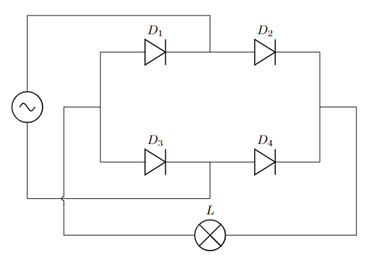
\includegraphics[width=\linewidth]{images/Montagefleche.png}

            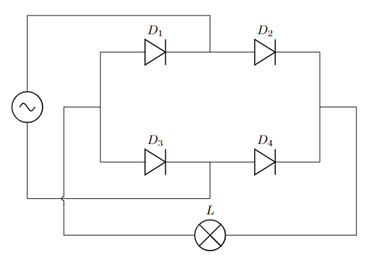
\includegraphics[width=\linewidth]{images/Montagefleche.png}
            
        \end{multicols}

        \item Préciser le rôle du chargeur de téléphone portable. 

        \cadreblanc{10}
    \end{enumerate}

\item Expérimentation 
  \begin{enumerate}[label=2.\arabic*.]
\item  Réaliser le montage ci-dessous en utilisant les réglages suivants : \\
\begin{itemize}
\item tension alternative de 6 V;
\item au moins 2 périodes visualisables sur l'oscilloscope;
\item l'amplitude sur l'écran la plus grande possible.

\end{itemize}
\begin{center}
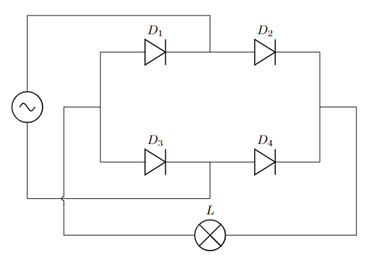
\includegraphics[scale=0.5]{images/Montagefleche.png} 
\end{center}
\item Brancher l’oscilloscope afin de visualiser la tension d’entrée \textbf{(avant le pont de diodes)}. 
\vfill
\fbox{Attendre l'accord de l'examinateur avant de mettre sous tension.} 

\vfill
\renewcommand{\arraystretch}{2.8}
\begin{tabularx}{12 cm}{|c||X|X|}
\hline

\includegraphics[scale=0.5]{images/appel exam.png}  & & \\[-0.7cm]
Appeler M Ruiz& Montage & Réglages\\
\hline 


 
\end{tabularx}
\vfill  
\newpage 

\item Représenter l'oscillogramme obtenu sur l'écran de l'oscilloscope. 



\begin{multicols}{2}
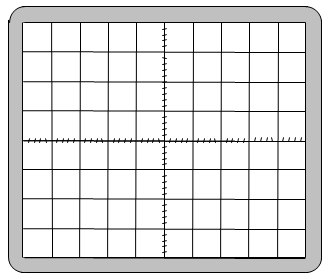
\includegraphics[width=\linewidth]{images/ecran oscillo.png} 



\renewcommand{\arraystretch}{2.8}
\begin{tabularx}{8 cm}{|c||X|X|}
\hline
Valeurs & $U_{Max}=$ & $T=$\\
\hline 
Calculs & $U_{Eff}=$ & $f=$\\
\hline
\end{tabularx}

\vfill

\end{multicols}

\begin{multicols}{2}
    \item Brancher l’oscilloscope afin de visualiser la tension de sortie (après le pont de diodes). \fbox{
\includegraphics[scale=0.5]{images/appel exam.png} 
Appeler M Ruiz}
\end{multicols}

\item Représenter l'oscillogramme obtenu sur l'écran de l'oscilloscope. 



\begin{multicols}{2}
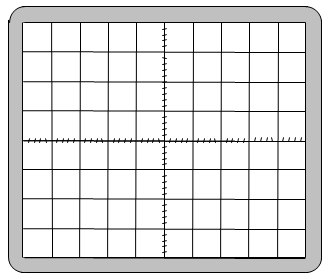
\includegraphics[width=\linewidth]{images/ecran oscillo.png} 



\renewcommand{\arraystretch}{2.8}
\begin{tabularx}{8 cm}{|c||X|X|}
\hline
Valeurs & $U_{Max}=$ & $T=$\\
\hline 
Calculs & $U_{Eff}=$ & $f=$\\
\hline
\end{tabularx}

\vfill

\end{multicols}


\item  Réaliser le montage ci-dessous : \\

\begin{multicols}{2}
    \centering
    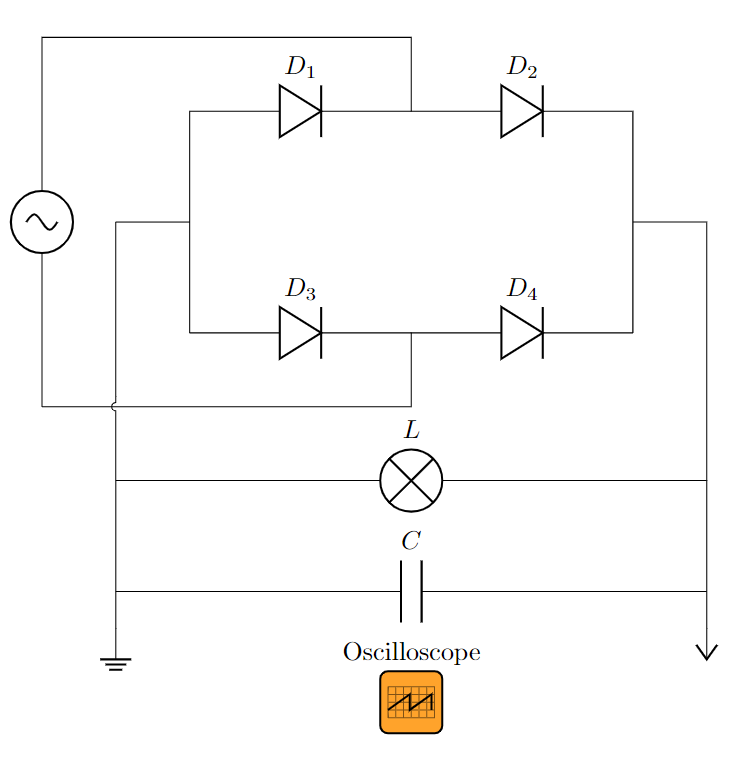
\includegraphics[width=\linewidth]{images/Montage - Pont.png} 
    
    \columnbreak
    
    \centering
    
\includegraphics[scale=0.5]{images/appel exam.png}
    
    Appeler M Ruiz
    
    \vspace{0.3cm}
    
    \renewcommand{\arraystretch}{2.8}
    \begin{tabularx}{\linewidth}{|c||X|X|}
        \hline
        Évaluation & Montage & Réglages\\
        \hline 
        & & \\
        \hline
    \end{tabularx}
\end{multicols}



\item Remplacer le condensateur de capacité ~$C=470 nF$ par un condensateur de capacité $C= 4 700 nF$ ; noter vos observations. 
\vspace{8mm}
\dotfill

\end{enumerate}

\begin{enumerate}[label=3.\arabic*.]
\item Déterminer, en V, la valeur de la tension U.
\vspace{8mm}
\dotfill 
\item De quel type de tension s'agit-il ? 
\vspace{8mm}
\dotfill 

\item Quel est le rôle du condensateur ? 
\vspace{8mm}
\dotfill 


\item Mesurer à l'aide d'un voltmètre la tension aux bornes de la lampe $L$ , noter sa valeur. \dotfill 

La valeur lue sur le voltmètre est-elle en accord avec la valeur trouvée à l'aide de l'oscilloscope. 
\vspace{8mm}

\dotfill 




\vspace{8mm}



\end{enumerate}


\end{document}